\section{Decompilation} \label{sec:existing-decompilation}
In general, IR with recovered variables and type information is more 
analysis-friendly, transformations and analyses provided by LLVM framework 
could be reused in an automatic way. Nonetheless, sometimes we still need to 
manually inspect the output of reverse engineering for better understanding (e.
g., malware analyses). In such cases, IR involving only simple arithmetic and 
memory operations is not conducive for human analysts to read and understand. 
Thus, decompilation is usually used as the last step of reverse engineering to 
transform IR into high-level programming languages. In this section, we will 
give a general discussion about decompilation techniques.


\subsection{Control Flow Structuring} \label{sec:existing-structure}
Based on the lifted high-level IR, the critical step to translate IR to 
programing language is control flow structuring. As shown in \F~\ref
{fig:structure}, CFG is first reconstructed from IR, then the structural 
analysis is employed to refine and summarize CFG nodes into high-level control 
flow structures such as if-then-else constructs and loops.

\begin{figure}[tb]
  \centering
  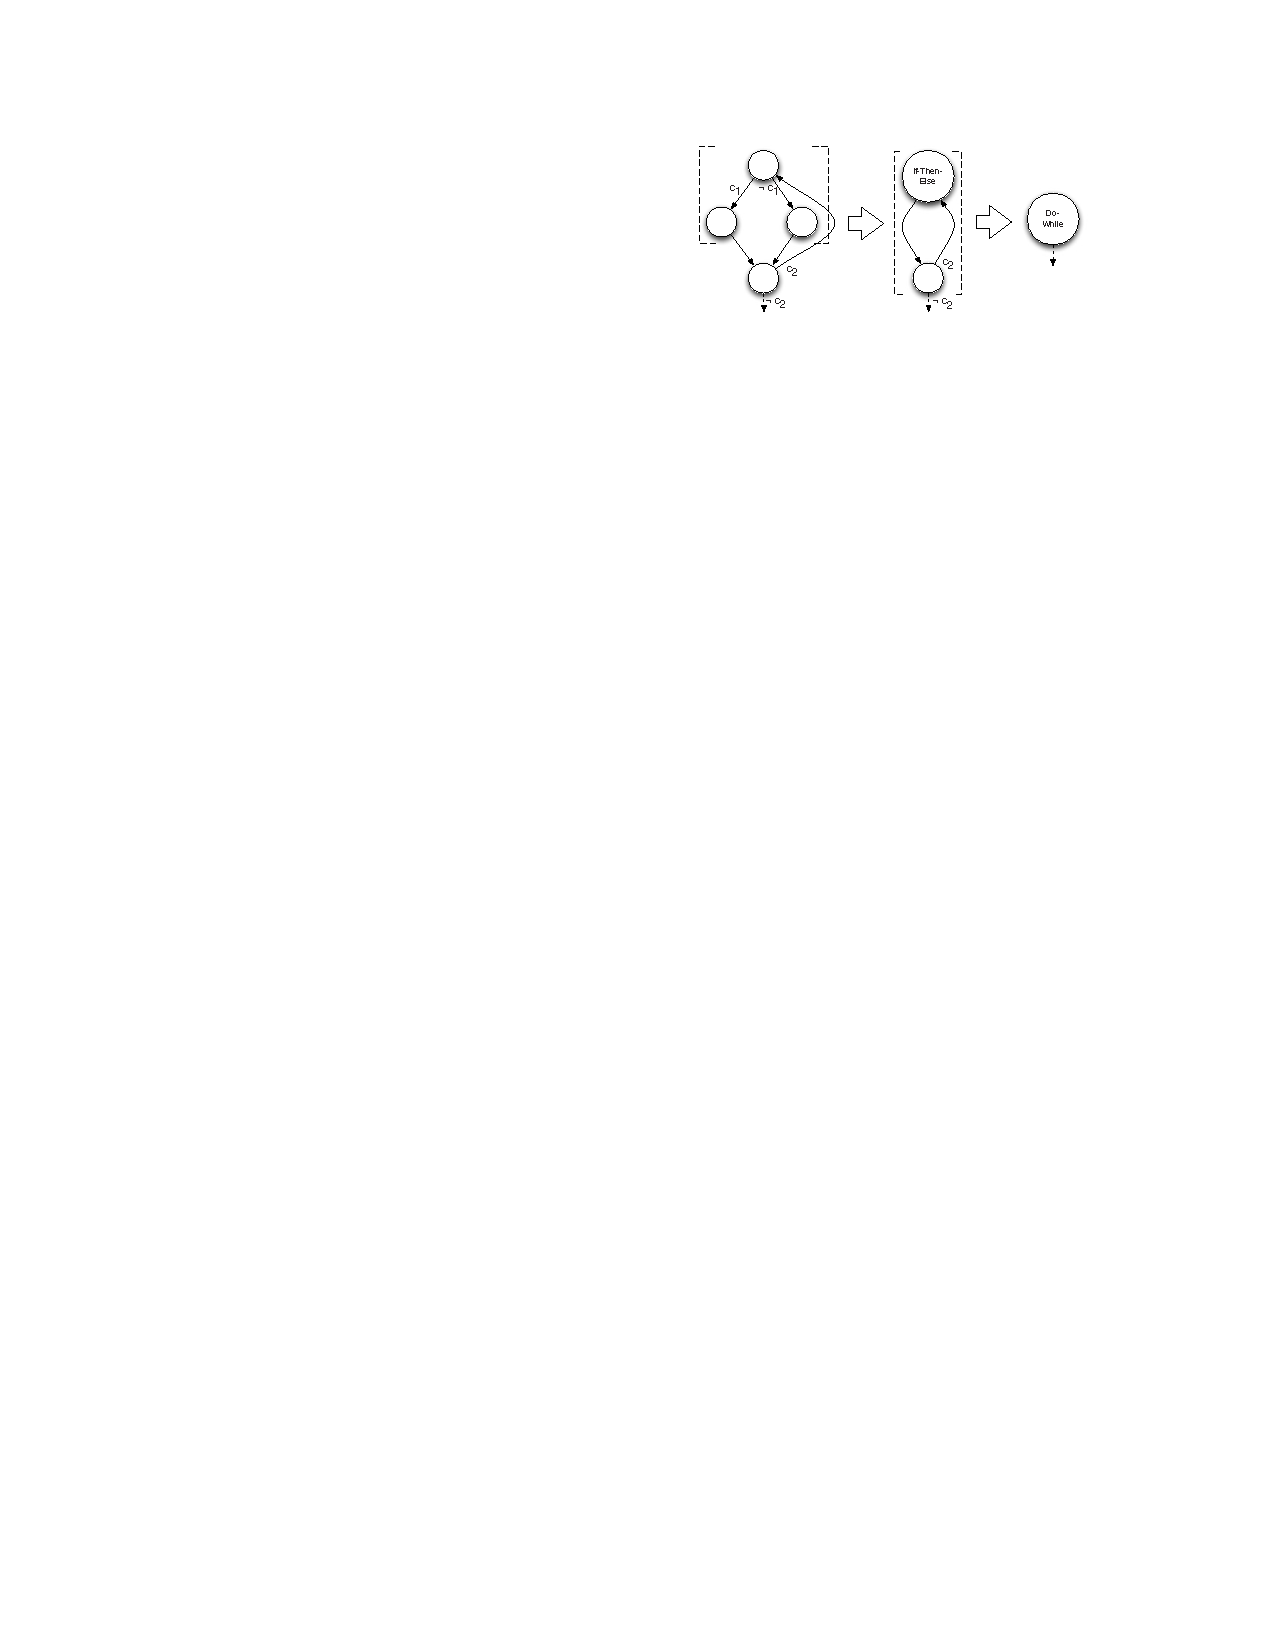
\includegraphics[width=0.6\textwidth]{fig/structure.pdf}
  \caption{Example of structural analysis.~\cite{brumley2013native}}
  \label{fig:structure}
\end{figure}

The recovered structure must be completely consistent with the semantics of the 
original program, thus Phoenix~\cite{brumley2013native} proposed \textit
{sematic-preserving} structural analysis that could be safely used in 
decompilation.
Phoenix uses manually crafted graph schemas or patterns to simplify a sub-CFG 
into a high-level structure, as illustrated in \F~\ref{fig:patterns}. These 
patterns will be iteratively applied for structuring. More specifically, 
Phoenix will iteratively remove an edge from the CFG by emitting a \texttt
{goto} statement until structuring can progress again.

\begin{figure}[tb]
  \centering
  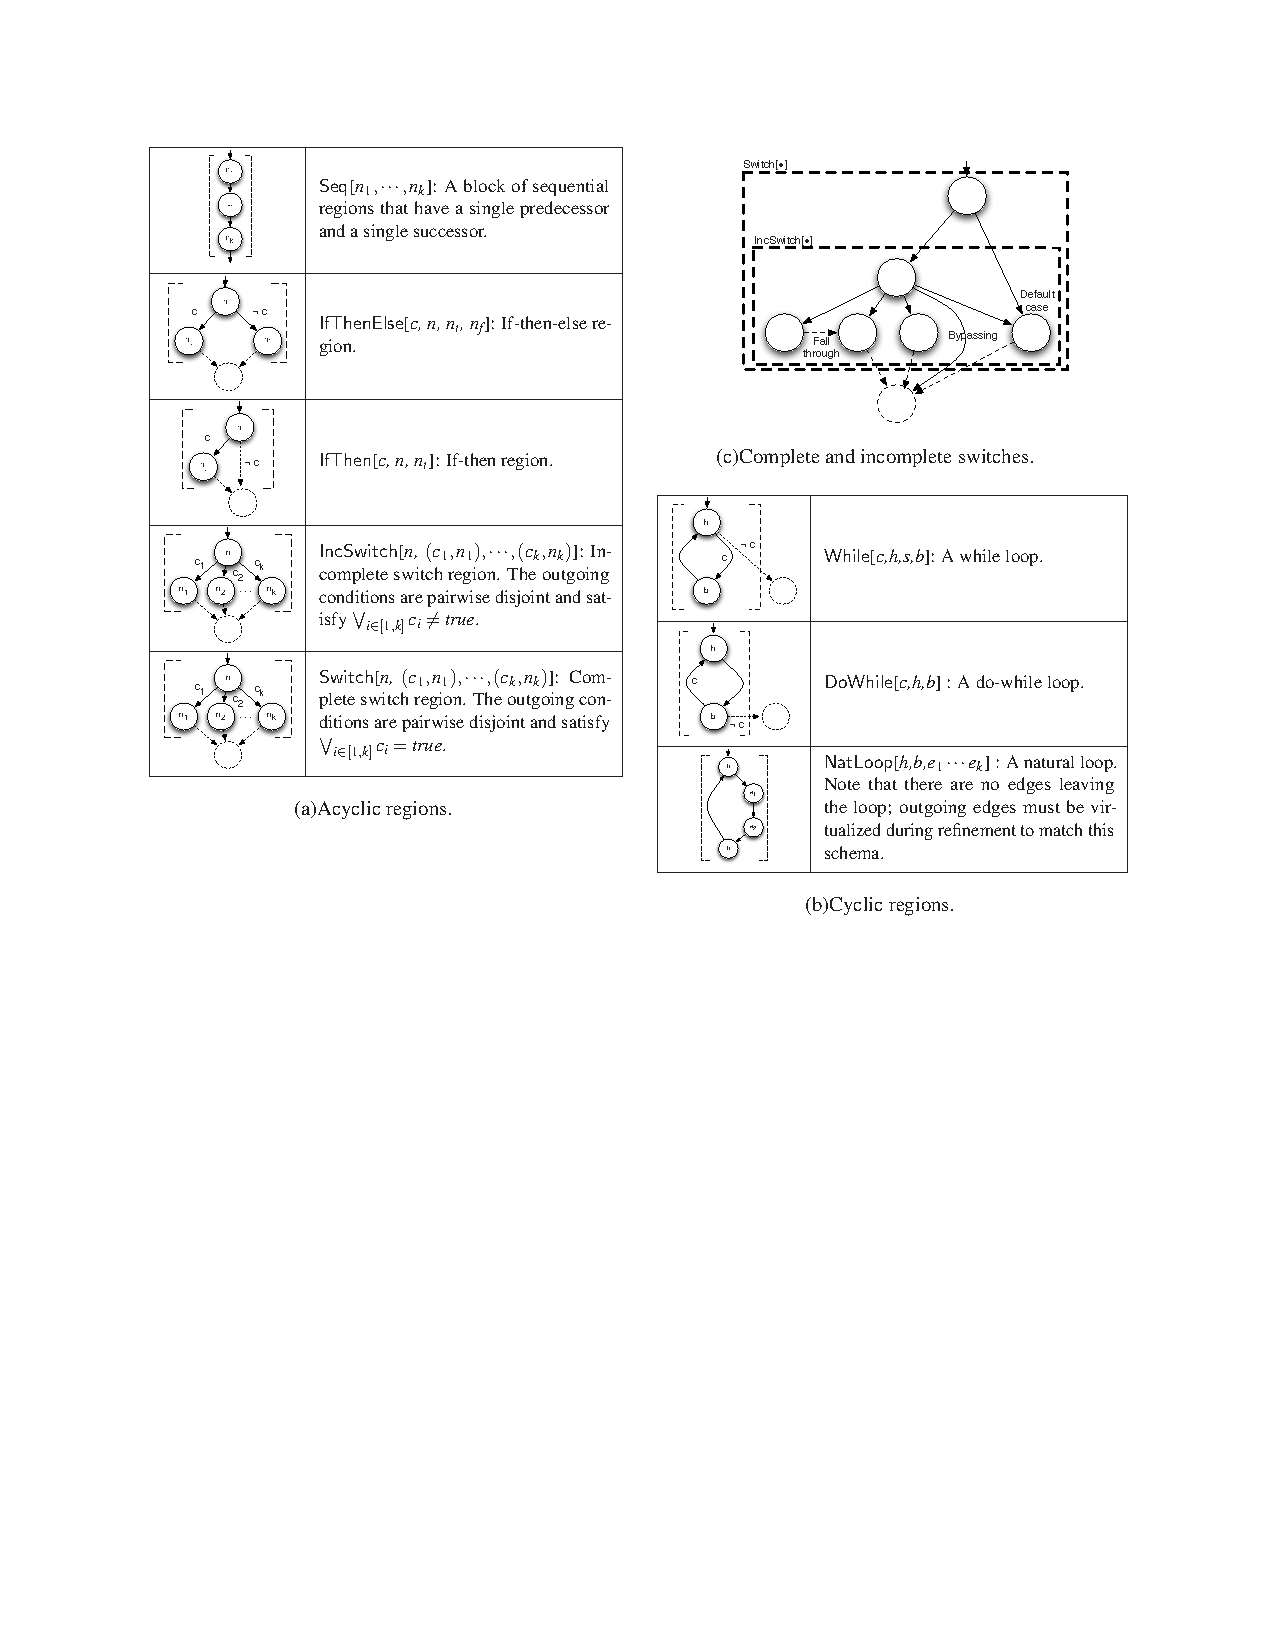
\includegraphics[width=0.8\textwidth]{fig/patterns.pdf}
  \caption{Semantics-preserving patterns.~\cite{brumley2013native}}
  \label{fig:patterns}
\end{figure}

On top of this idea, \textsc{Dream}~\cite{yakdan2015no} extends the structuring 
technique with \textit{sematic-preserving transformations} that transform 
cyclic subgraphs with multiple entries or multiple successors into semantically 
equivalent single-entry single-successor (acyclic) subgraph. Even more, \textsc
{Dream} presents a \textit{pattern-independent} structuring algorithm that is 
able to recover all high-level control constructs in acyclic regions. With 
these two techniques, Dream can produce \texttt{goto}-free structured 
decompiled code. Apart from that, \textsc{Dream} also produces more compact 
code compared with Phoenix and the \textit{de facto} industrial standard 
decompiler Hex-Rays~\cite{hex2014ida}.

\subsection{Meaningful Variable Names Recovery} \label{sec:existing-var-names}
Besides the structuring techniques that are essential to the correctness of 
decompiled code, another line of research attempts to recover variable names 
from decompiled code. For example, DIRE (Decompiled Identifier Renaming Engine)
~\cite{lacomis2019dire} uses an encoder-decoder network to reconstruct 
semantically meaningful variable names based on the lexical and structural 
information produced by the decompiler. While this method does not change the 
semantics of decompiled code, it can highly increase code readability by 
achieving 74.3\% accuracy in predicting variable names on more than 164k 
programs collected from Github.

\subsection{Neural Program Decompiler} \label{sec:existing-neural-dec}
With the rise of machine learning, the neural network is also used for 
decompilation.  As an end-to-end neural-based framework for code decompilation, 
Coda~\cite{fu2019coda} tries to get the decompiled code from assembly code 
directly without solving the challenges we discussed in Chapter \ref
{sec-challenges}. Coda uses an instruction type-aware encoder and a tree 
decoder to generate an abstract syntax tree (AST) as the code sketch, then 
updates the code sketch using an iterative error correction machine guided by 
an ensembled neural error predictor.
%
However, Coda did not compare their results with the best available decompiler, 
IDA~\cite{hex2014ida}. Instead, they compare with an open-source decompiler 
named RetDec~\cite{retdec}, which cannot represent the state-of-the-art 
decompilation techniques. More importantly, although Coda claims to be able to 
preserve both functionality and semantics, the \textit{Token Accuracy} metric 
they used does not involve semantic or functional checks. Therefore, at this 
point, we consider that neural network techniques are not ready for the 
end-to-end decompilation task, given the existing technical conditions. 
However, we believe that neural networks still have great potential for solving 
specific problems in software reverse engineering tasks, such as variables 
recovery and function boundary identification.

% \fixme{Do we need to discuss Fucntion recovery? RNN based decompiler? }
